\cleardoublepage
\singlespacing
\chapter{SYSTEM DESIGN}
\label{c:design}
\doublespacing\nointerlineskip

The design for WuKong fault tolerance system is guided by the goals and
challenges outlined in chapter~\ref{c:intro}: We want fault tolerance
policy to be expressive, component specific, yet decoupled from physical
hardware specifications so it will work with a range of network configurations.
Furthermore, we want a reconfigurable redundancy architecture for
service-oriented heterogeneous WSNs so components would be resilient to partial
failures and degrade gracefully as indicated in the policy while being efficient
and simple in terms of engineering design.

\section{User Preference for Fault Tolerance}

\begin{figure}[h!]
\centering
    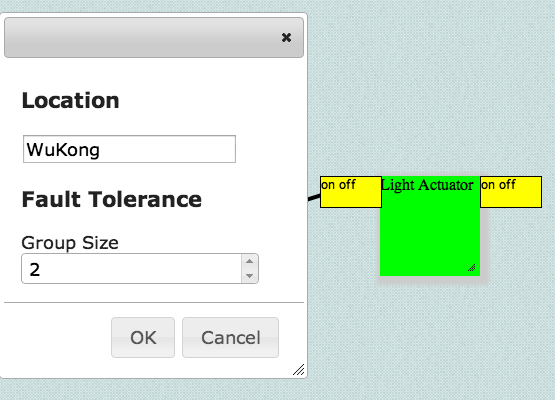
\includegraphics[width=\linewidth]{figures/fbp-policy}
\caption{An example of categories a user policy could impose on a component}
\label{fig:fbp-policy}
\end{figure}

\begin{figure}[h!]
\centering
    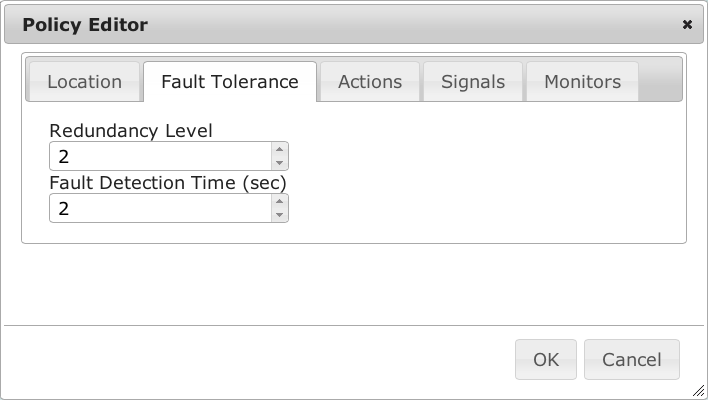
\includegraphics[width=\linewidth]{figures/fbp-ft-policy}
\caption{An example of fault tolerance policy}
\label{fig:fbp-ft-policy}
\end{figure}

% What is user policy, What is it for, how does it influence the system
User policy guides the decisions and achieves certain outcomes for the system.
Specifically, user policy controls how the system could behave in high level
concept.
When users starts up WuKong user interface, they will be confronted with the
application where users could specify policy for each application component on,
for instance, specific location the application component should be mapped to,
or number of redundant devices the application component would have as
illustrated in figure~\ref{fig:fbp-policy}.

% What are fault tolerance policy
Users are also capable of specifying fault tolerance requirements via the
user policy for fault tolerance as shown in figure~\ref{fig:fbp-ft-policy}
Redundancy level indicates the number of devices that will be able to take over
when the service failed. Fault Detection Time represents the time the system
should take at most to detect an failure in seconds.

There are timeouts set accordingly to prevent deviation in wireless communication quality,
internal crystal clock to reduce the chances of getting false positives. Right
now there is no way to find the correct timeout for the network, so we set it to
right around 2x times of the heartbeat period we set fo the network.

\section{Deploying Application with Fault Tolerance}

In WuKong, deployment consists of discoverying available resources and network
topology, converting application from high-level abstractions to low-level
machine instructions, then determine the parameters based on user policy,
finally combine all together and deploy to the network. The process was briefly
described in section~\ref{c:background}, however, the thesis has made some
significant changes to the process to support strip, an redundancy abstraction
used in failure recovery and reconfiguration algorithms. First, we add a new
process in mapper to take the routing topology results in discovered network
info, so we could know the neighbors for each device. Next we take the existing
mapping process, and convert it to outputting strips. So instead of one-to-one
mapping from components to devices, now each component maps to a strip, which
could be seen as a list of devices supporting such service ordered by the
ordering function used. The default ordering function uses first-fit in a first
come first process fashion, thus the ordering of the strip is randomized, as it
depends on the order of processing.

An first-fit algorithm for mapping is shown in algorithm~\ref{alg:mapping}

\begin{pseudocode}[framebox]{FirstFitComponentToStripMapping}{S, F}
\label{alg:mapping}
C \GETS {S}\\
X \GETS {F}\\

\FOREACH c \in C, x \in X \DO
  \BEGIN
    \IF c \in x \THEN
      \BEGIN
        c << x\\
        \COMMENT{Append x to c}
      \END\\
  \END\\

\RETURN C
\end{pseudocode}

S is the set of components, F is the set of
sets each represents a network node with service capabilities. This algorithm
will produce a mapping of C, a set of lists in first-come-first-serve order.

Once the mapping is produced, each device would be reprogrammed to create
corresponding WuObjects to host the services.

\section{Strip}
\label{s:ss}

\begin{figure}[h!]
\centering
    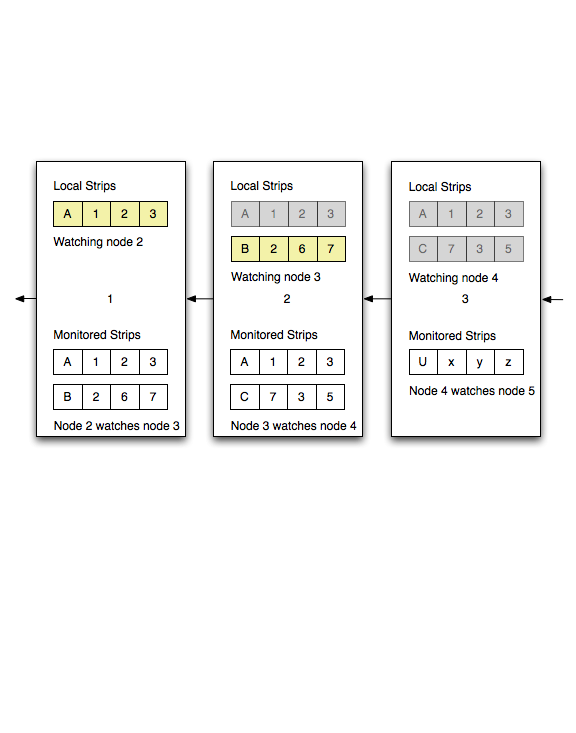
\includegraphics[width=\linewidth]{figures/strip1}
\caption{An example network with several strips}
\label{fig:strip1}
\end{figure}

Representing a component in WuKong application, each Strip contains a list of
node on which the WuObjects representing the component are hosted. As seen from
the figure~\ref{fig:strip1}, each node represented by a big white block contains
a copy of strips for components that are specified to have redundancy in fault
tolerance policy. Nodes holding a duplicated WuObject are members of the strip.
The membership of a strip is called the view. Only the WuObject hosting at the
head of the strip will be active, while the rest are backups.  As seen from
figure~\ref{fig:strip1}, node 1 has a active WuObject for component A as shown
highlighted in yellow, but duplicated WuObjects A in node 2 and 3 are inactive
in grey. In Strips, when one member failed, the next one will take over. For
instance, if a strip is constructed like this $\rightarrow 1-2-3-4-5$, when
3 failed 4 will take over the place of 3, and the new chain will look like this:
$\rightarrow 1-2-4-5$. Now if 1 failed, 2 will take over which would result in
$\rightarrow 2-4-5$, since node 2 is now at the head of the strip, its WuObject
will be active. 

Typically, there would be multiple components deployed to the network and each
node could carry multiple WuObjects, therefore many of these strips in the
network would crisscross with one and others. It is not unlikely to see a node
carrying active and inactive WuObjects at once.

\section{Reconfigurable Redundancy Architecture}

Once the application is deployed, each target device would host one or many
WuObjects where each represents a service for an application component. However,
the network has to be resilient to failures, it has to detect and recovery
autonomously. In the following paragraphs, we will be describing the subsystem
which is used to support failure detection and recovery.

\subsection{Decentralized Failure Detection}
\label{s:dfd}

We want the heartbeat protocol to able to reach the entire network so any
failures will be detected. In order to avoid single point of failures, the
protocol will have to be decentralized, thus the failure one of component would
not bring the whole failure detection system down.

%Note to self: mention single-hop, multi-hop in limitations or future work
Distributed failure detection enables high-availability in distributed systems
where partial failures is rather common.  We utilize heartbeats to detect
failures, a common technique widely used to detect failures in high-availability
distributed systems.  Heartbeats are messages sent periodically until it's
unable to send messages anymore. Each node is therefore suspected dead when
others stopped receiving messages from it after an extended period of time.
Nodes were assumed to fail by stopping and will never come back.

There are abundant literature on designing heartbeat protocols to ensure
high-availability for distributed systems. Our work employed a heartbeat
protocol arranged in such as way where each node sends a heartbeat to the
previous node and the last node sends back to the first node forming a daisy
chain as represented by the black arrows in figure~\ref{fig:strip1}.

To prevent tight coupling and redundancy in heartbeats, strips are separated
from heartbeats so the order of the strip does not affect the ordering of
heartbetas and vice versa. The heartbeat protocol is a support layer below
strips, the layers above will take advantage of the given information from the
layer below to recover the system.

\subsection{Failure Recovery}
\label{s:fr}

When a failure is detected, there are two tasks that the system would have to do
to recover from failures. First it has to make sure all members that carries
the strips in the failure nodes will have consistent view of the strips.
Second, it would need to propagate the changes to reconfigure other parts of
the system that depend on the locations of the heads of the affected strips in
order to function. The details of each task is described in the following
sections.

\subsubsection{Consistent view of strips}

\begin{figure}[h!]
\centering
    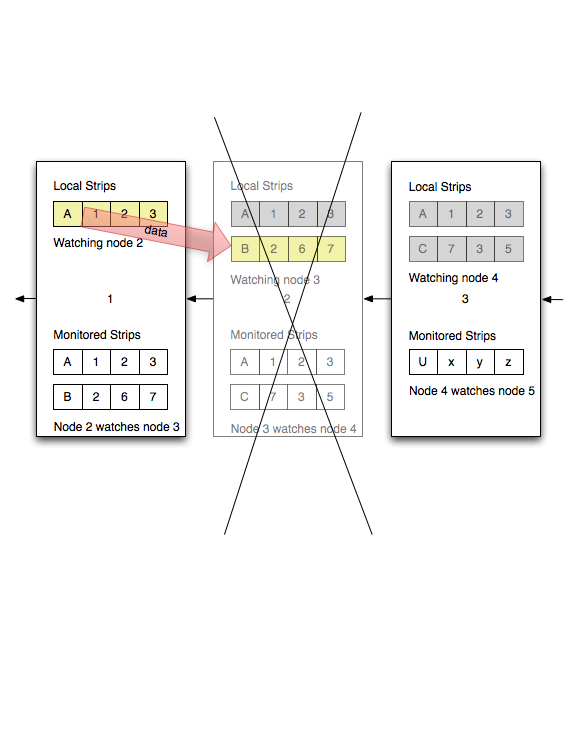
\includegraphics[width=\linewidth]{figures/strip3}
\caption{A failure occurred at node 2 in the network}
\label{fig:strip3}
\end{figure}

Consistent view of strips is required to pick a replacement node in the event
of failure. Without consistent view, nodes will not be able to know if the
component has been replaced.
For example, in figure~\ref{fig:strip3}, when node 2 failed, node 1 will detect
this, but without algorithms to maintain consistency, node 3 would not be
certain if node 1 or 2 are still alive, thus it might take actions that could
compromise the network.

But detector might not know which strips the monitoring node is a member of, so
every node will have a copy of its monitoring node's strips view as shown in
figure~\ref{fig:strip1} below the "Monitored Strips" section where node 1 has
knowledge of the strips views of its monitoring node 2.

% TODO: better to have a figure here to explain view update

The detector of the failure would initiate the recovery algorithms.
Since the detector will be responsible for recoverying for the failed node,
every node needs to have membership knowledge of the strips from the nodes it
is monitoring. For example, if node A is monitoring node B, A would know the
members of all strips in node B in addition to its local strips. Strips only
specifies the order of recovery, it is not correlated with the network
structure for the fault detection, in other words, a strip with A and B doesn't
mean B is monitoring A, as B could be monitored by C which depends on the
structure of heartbeat protocol layer.
In the initial algorithm, the detector node will prepare a update message to
inform all members of the strips with which the failed node is associated with.
Assuming that every node that monitors other node will have knowledge of the
strips that it contains and the members that the strips pertain. The node would
send out a marker message first to confirm the nodes which are still
functioning, and once all acknowledges have been received, it will proceed to
send the update message to update their local knowledge of the strips to reach
a consensus. The ordering of the messages wouldn't matter since the end state
of any failure sequence for any strip would be the same. For example, given
a strip of three members $\rightarrow 1-2-3$, if the updated failure sequence
is given in any permutation by $[1, 2]$ or $[2, 1]$, the end results would be
the same $\rightarrow 3$ since the remaining members from those two failure
sequence is the same and the relative order of the members would stay the same.
\begin{comment}
Let's assume there is a pair of failure patterns with the same members but
different orders that would do update operations on the same strip but would
leave the strip in different results. If that's true, then by building back the
strips from the result in the order of update operations would result in
a different starting state, that implies the strips have different members or
member orders to start with, a contradiction.
\end{comment}
Therefore there is no need for extra communication overhead to maintain
ordering to gaurantee level of consistency between members since they will all
come to the same conclusion given each receiver receive the same messages. The
overhead are messages required to update each member's internal membership
information.


\subsubsection{Reconfiguration}
\label{s:reconfig}


Even though consensus of the new view for each strip in the failure nodes has been
reached, other devices in the network with connected components would also need
to be updated. 

The detector after finishing synchronizing views, will initiate
the reconfiguration algorithm. First, the initiator will identify application components
that are connected with the components carried by the failed device (linked in the
FBP). Then initiator would issue the update message to each head of the strips of the connected components
to reconfigure the new heads of the affected strips.

As shown in figure~\ref{fig:strip7}, node 1 with its updated view of the strips
after the failure of node 2 would need to update the new head of component A,
which is still node 1 in this case, with the new head of compoennt B since
component B is connected to compoennt A; node 1 also needs to update the new
head of component B with the new head of component A as well. Thus node 1 will
send a reconfiguration message to node 1 and node 6 about the changes in both
heads of component A and component B.

To keep the nodes updated after reconfiguration, as most services in WuKong
applications does not store any past data, the devices with connected components whose WuObjects
originally are sending data to the WuObjects on the failed devices would force a data push to
bring the new heads up to date, and vice versa, so instead the devices with
connected components whose WuObjects originally are receiving data from the
failed devices would force a data pull.

The detector needs to update its knowledge of the "Monitored" section after
reconfiguration. The detector knows which node the monitoring node is
monitoring, it will send a update heartbeat message request and instruct it to
send heartbeats to itself, then it will send a request for its knowledge of
local section and update its "Monitored" section, both the strips and the node
it is monitoring. As illustrated in figure~\ref{fig:strip9}, node 1 will get
updated with the heartbeat information from node 3, which is monitored by node
2. And also in figure~\ref{fig:strip10}, node 1 will also get updated with the strip
information from node 3.


\begin{figure}[h!]
\centering
    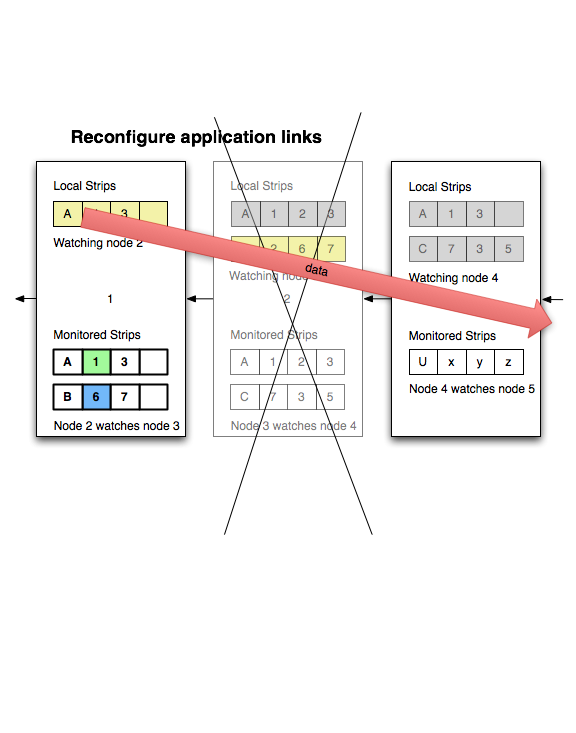
\includegraphics[width=\linewidth]{figures/strip7}
\caption{Reconfigure application links}
\label{fig:strip7}
\end{figure}

\begin{figure}[h!]
\centering
    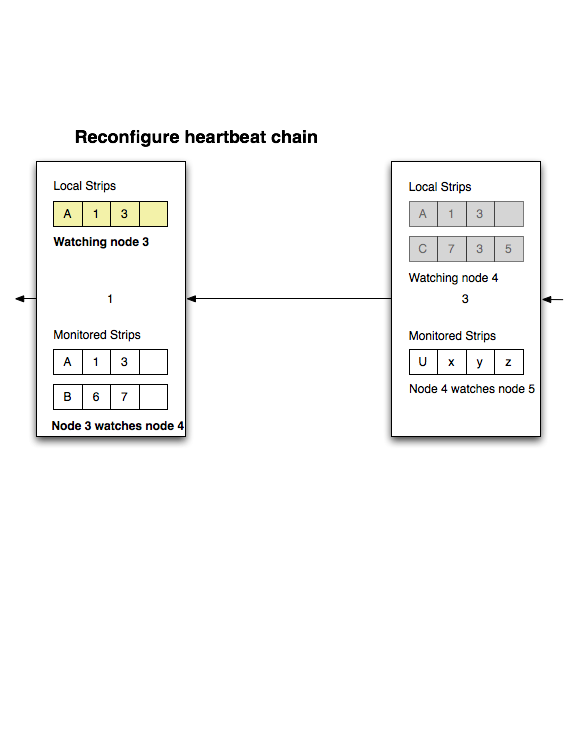
\includegraphics[width=\linewidth]{figures/strip9}
\caption{Reconfigure heartbeat protocols}
\label{fig:strip9}
\end{figure}

\begin{figure}[h!]
\centering
    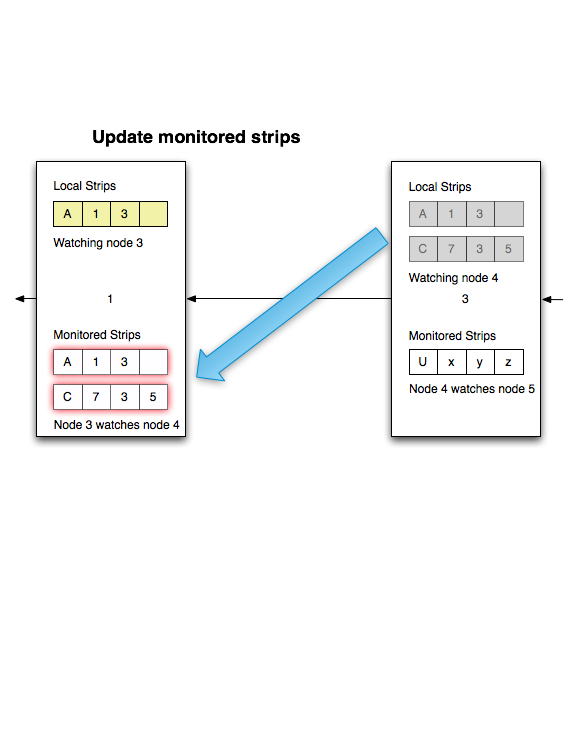
\includegraphics[width=\linewidth]{figures/strip10}
\caption{Update monitored information}
\label{fig:strip10}
\end{figure}

\section{Complexity Analysis}

% Complexity analysis
% TODO:Just pasted, need revision
The lower bound of message overhead for heartbeats arranged in a daisy chain
loop in a network of size n is $\Omega(n)$, the upper bound is also $O(n)$, since
there is only one message sent by a node at any given moment.

% Complexity analysis
% TODO:Just pasted, need revision
For an application with m components deployed to a network with n nodes where
$n > 1$, the lower bound of memory overhead of the strips for a random member in
the network is $\Omega(1)$ since a node must carry at least one strip and lowest
member requirement of a strip is 2. The upper bound is $O(m*n)$ since the strips
could span the whole network. But in reality, since the nodes typically have
fixed memory and fixed capability for the duration of the lifetime in the
network, the upper bounds cannot grow indefinitely. The memory overhead a strip
could impose on a node is determined by node's capability and memory size.


% Complexity analysis
% TODO:Just pasted, need revision
The lower bound of message overhead by the reconfiguration protocol
with one node failure in the same network is $\Omega(1)$, since if there is only
one component with 2 members on the failed node, the detector would only need to
send 1 messages to the remaining strip member of the failing node, and none if
the component is not connected to any other components, and finally 1 more
message to get the information from the nodes monitored by the failed node. The
upper bound is $O(n + m)$ since if the failed node carried m components where each
strip contains n members, the detector would have to send (n-2) messages to all
functioning members of the m strips carried excluding itself plus the messages
to all other strip heads connected to the failing node. 

The time to recover highly depends on the messages sent for the reconfiguration
and the detection time. The lower bound is $\Omega(1)$ with the same assumption
with constant component and members, but the upper bound is $O(b + n + m)$ where
b is the heartbeat period.

The cost for time for recover is the time itself. Time is the overhead. Thus the
longer time it take to recover the higher the overhead. By setting a shorter
heartbeat period, it would take a shorter time to recover, thus a lower
overhead. I assume every message takes at least a fixed amount of time, and
there need at least amount of messages to recover, so the more messages it takes
to recover, the longer the time it will take to recover. Here it is assumed that
heartbeat messages are never lost/dropped, and in-node computation take
negligible amount of time thus it is ignore. %If it is about the message overhead within a certain time period, then of course the higher the period the lower the message overhead.

